在对源文件进行了足够的检查、变换并且提取了足够的信息后,应当具备了以下条件:
\begin{itemize}
	\item 确保源文件语法、语义正确
	\item 有一个同目标汇编码接近的中间表示
	\item 有一个能够查询标识符(包括源文件中的符号和中间表示中的临时变量)信息的接口
\end{itemize}
接下来就可以开始生成目标代码了,我们将在这一章介绍编译器观点下的作为目标机器的Unicore32体系结构、MiniC将三元式表示翻译成Unicore32汇编语言的过程以及MiniC在目标代码上进行的机器相关优化。
\section{编译器-目标机器二进制接口}
\label{target_machine}
本节介绍编译器视角下的Unicore32体系结构,主要包括寄存器使用情况和内存的维护(包括栈帧和全局区)。

{\it \anchor 有关Unicore32指令系统,请参阅:《Unicore32处理器ISA(子集)介绍》}\\

\subsection{寄存器使用情况}
下表对照了UniCore32的寄存器使用规范和MiniC的寄存器使用情况:
\begin{center}
	\begin{tabular}{|l|l|l|}
	\hline
		寄存器 & Unicore32寄存器使用规范 & MiniC \\
	\hline
		r0-r3 & 传递参数;r0保存返回值 & 传递参数;r0保存返回值;在函数内用于无寄存器变量的装入和运算 \\
	\hline
		r4-r15 & caller save & caller save,个数可调$^*$\\
	\hline
		r17-r25 & callee save & callee save,个数可调$^*$\\
	\hline
		r26 & 静态基址 & 装入全局变量地址\\
	\hline
		r27 & 栈帧基址 & 栈帧基址\\
	\hline  
		r28 & 调用者SP & 传参时用于装入和运算(由于此时r0-r3不能用于运算);生成立即数\\
	\hline 
		r29 & 栈基址 & 栈基址 \\
	\hline
		r30 & 返回地址 & 返回地址 \\
	\hline 
		r31 & PC & PC \\
	\hline
	\end{tabular}
	\label{registerstat}
\end{center}
{\it $^*$\verb|register_stat.h|用于调整可用的caller save和callee save寄存器的个数}

注意到r28的用法和规范有差异,但这不影响MiniC生成的目标文件同其它Unicore32编译器生成的目标文件的链接。
\subsection{内存的维护}
\subsubsection{栈帧的维护}
在程序运行之初,装载器给r29赋初值后,维护栈帧的工作交由程序自己来进行。因此编译器需要在目标代码中添加相关代码。

栈帧维护的汇编语句将在翻译表示函数调用的三元式(\verb|param|和\verb|call|)时产生。

下图左图展示了函数调用时栈帧的情况,右图展示了局部数组的保存方法:
\begin{center}

\begin{minipage}{0.4\textwidth}
\begin{center}
	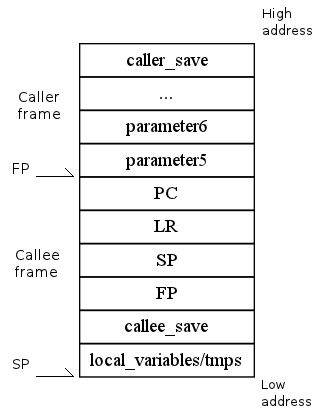
\includegraphics[scale=0.6]{stack_frame.png}
	\label{fig:stackframe}
\end{center}
\end{minipage}
\begin{minipage}{0.4\textwidth}
\begin{center}
	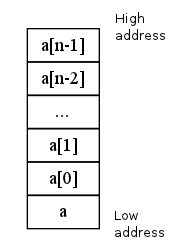
\includegraphics[scale=0.6]{local_array.png}
	\label{fig:localarray}
\end{center}
\end{minipage}
\captionof{figure}{栈帧与局部数组示意图}
\end{center}
FP以上(高地址方向)是调用者的部分栈帧(略去部分和被调用者栈帧相似),其中保存了call save寄存器以及传给被调用者的从第5个到最后一个参数(如果被调用者参数小于等于4,那么省去这一段)。

FP到SP的一段是被调用者的栈帧,其中保存了调用时的PC,返回地址,调用者的栈顶地址和栈帧基址以及callee save寄存器的值。同时,每一个局部变量和没有分配寄存器的临时变量在栈帧中均有位置。

对于局部数组,数组的头指针存放在数组起始的第一个字节,即不考虑对齐的情况下一个$4n$字节的\lstinline|int|数组将占用$4n+1$的空间。

\subsubsection{全局区的维护以及大立即数的处理}
我们将全局变量(或数组)、字符串常量保存在全局区中。由于全局区可能较大,使用基址和偏移量的寻址方式很可能出现偏移量过大不能使用带立即数的访存指令的问题。为此,我们将每个函数需要用到的全局变量的指针保存在该函数的代码段末尾,并分配给它们一个标号。当使用这些标号寻址时,汇编器会自动将寻址方式转换成PC相对寻址。

对于无法使用立即数寻址的三元式中的立即数,我们也将它保存在函数的代码段末尾,通过PC相对寻址将其读入。

例如下述代码:
\begin{lstlisting}
int a,b;
int f()
{
	a=25500;
	b=25500;
}

\end{lstlisting}
我们将生成如下的汇编代码:
\begin{verbatim}
	.comm	b, 4, 4
	.comm	a, 4, 4
	.text
	.global	main
	.type	main,function
main:
	@Create stack frame
.L1:
	ldw	r3, .L3+8
	ldw	r1, .L3+0
	stw	r3, [r1+], #0
	ldw	r3, .L3+8
	ldw	r1, .L3+4
	stw	r3, [r1+], #0
	@End of program
.L3:
	.word	a
	.word	b
	.word	25500
\end{verbatim}
\section{寄存器分配}
\label{registeralloc}
Unicore32采用RISC结构,具有31个通用寄存器,所以对于大部分程序,几乎所有变量都可以保存在这些寄存器中,以减少对内存的读写。因此需要一个方法来给每个变量关联一个寄存器,该方法需要保证能用最节约的方式分配,同时变量之间不能互相污染。

MiniC采用了启发式的图染色寄存器分配算法。该算法依赖于在三元式上进行的活跃变量分析的结果,即需要在某个程序点上每个变量的活跃信息,然后建立一个干涉图$G(V,E)$,其中$V$是变量的集合,$(v_1,v_2)\in E$当且仅当存在某个程序点,使得在此处$v_1$和$v_2$同时活跃。给变量分配寄存器就相当于给这张干涉图着色。

举例如下,对于左图的三元式序列(花括号中是该句处的活跃变量),干涉图为右图:
\begin{center}

\begin{minipage}{0.4\textwidth}
\begin{center}
	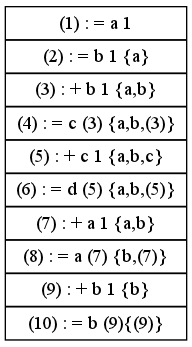
\includegraphics[scale=0.6]{register_allocation_triple.png}
	\label{fig:registerallocationtriple}
\end{center}
\end{minipage}
\begin{minipage}{0.4\textwidth}
\begin{center}
	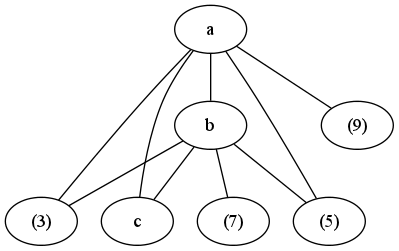
\includegraphics[scale=0.6]{interference_graph.png}
	\label{fig:interferencegraph}
\end{center}
\end{minipage}
\captionof{figure}{寄存器分配示例}
\end{center}
下表给出了不同的可分配寄存器数目的寄存器分配的结果:
\begin{center}
	\begin{tabular}{|l|l|l|}
	\hline
		变量 & 2个可用寄存器 & $\geq$3个可用寄存器 \\
	\hline
		a & 保存在内存 & r6 \\
		b & r5 & r5 \\
		c & r4 & r4 \\
		(3) & r4 & r4 \\
		(5) & r4 & r4 \\
		(7) & r4 & r4 \\
		(9) & r4 & r4 \\
	\hline
	\end{tabular}
	\captionof{table}{寄存器分配示例}
\end{center}
注意到在只有2个可用寄存器时,出现了寄存器不足的情况。对于这种情况MiniC会选择将某些变量保存在内存(即在干涉图中删除该顶点)。这些保存在内存的变量每次引用都需要读取内存;每次赋值都需要写入内存。在\cite{sunjiasu}中介绍的算法采用的选择策略是总选择度数最大的点删除,但是在一些对数组频繁操作的程序实例(如排序算法)中,采用这种策略将会使得数组基址被保存在内存中,使得每次读取数组元素之前要先读取基址,大大影响了性能。我们认为可以采用一种更为折衷的办法:综合考虑变量的使用频率和它的干涉边数,给出一个权衡后的解。但由于时间关系,这一想法没有实现。\\
{\it \anchor 有关寄存器分配和活跃变量分析的代码,请参阅:\verb|register_allocation.c|, \verb|live_var_anal.c|}\\
%TODO:三元式转换为目标代码
\section{将三元式转换为目标代码}
\label{tripletotarget}
\subsection{控制流语句的翻译}

\subsection{寄存器保护与同步}
\label{registerprotect}
\subsection{立即数的处理}

{\it \anchor 有关三元式转换为目标汇编码的代码,请参阅:\verb|gen_target_code.c|}\\
\section{机器相关优化}
\label{depopt}
在生成目标代码的过程中,我们已经对一些潜在的代码冗余进行了清理,但是受到中间表示和翻译方法的限制,生成出的目标代码仍有改进的余地,下面介绍我们在目标代码上,配合Unicore32指令系统进行的优化。
\subsection{窥孔优化}
\label{peephole:target}
{\it \anchor 有关目标代码上的窥孔优化的代码,请参阅:\verb|peephole.c|}\\
\subsubsection{合并访存语句}
如\verb|a[i] = 1|这样的MiniC语句翻译成的三元式如下:
\begin{center}
	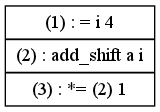
\includegraphics[scale=0.50]{merge_ldst.png}
	\captionof{figure}{合并访存语句示例}
	\label{fig:mergeldst}
\end{center}
根据三元式生成的目标代码为(假设r4中保存着a的基址,r5中保存着i的值):
\begin{verbatim}
add r5, r4, r5<<#2
mov r3, #1
stw r3, [r5+], #0
\end{verbatim}
由于Unicore32提供了“寄存器位移读取(写入)”的指令,这个操作事实上只需要:
\begin{verbatim}
mov r3, #1
stw r3, [r4+],r5<<#2
\end{verbatim}
由于\verb|add|和\verb|stw|可能不连续,逐句生成目标代码时,发现合并的可能较为困难,因此我们扫描生成出的代码,将所有符合上面例子中的情况都进行了合并。

这项简单的优化在循环地对数组访问的情况下对性能的提升比较明显。
\subsubsection{消除冗余的\lstinline|mov|}
由于三元式的一些局限,翻译得到的目标代码在读取内存操作的附近可能会有一些冗余的\verb|mov|语句,本优化类似于复写传播,目的是将这些\verb|mov|删除。

能被删除的\verb|mov|具有以下条件:
\begin{itemize}
	\item 从mov指令的源操作数最近的一次定值开始,到mov指令之间没有对mov的目标操作数引用。
	\item 从mov指令开始,将mov指令的源操作数替换为目标操作数时不会产生冲突。
\end{itemize}
\paragraph*{算法}
\begin{enumerate}
\item 对目标代码划分基本块(以跳转指令为标志),并在基本块上做一个简单的跳转关系图,每个基本块中记录每个它接下来可能执行的基本块。
\item 扫描代码。对每个mov语句,其目标寄存器为$Rd_{mov}$,源寄存器为$Rm_{mov}$。从该条语句向上寻找最近一条语句i,语句i的目标寄存器为$Rm_{mov}$。(语句$i$对$Rm_{mov}$定值)
\item 判断语句$i$是否可以被删除。原则有:
	\begin{itemize}
		\item 若$mov$语句到语句i之间有对$Rd_{mov}$的引用,则不可删除。
		\item 从语句$i$开始,根据跳转关系图向后扫描代码(深度优先的遍历)。若进入循环块则停止,语句$i$不可删除。
		\item 扫描过程中,若某调语句引用了$Rm_{mov}$,则将它替换为$Rd_{mov}$。若某条语句对$Rm_{mov}$定值,则这条扫描路径终止。若某条语句对$Rd_{mov}$定值,并在这之后又引用$Rm_{mov}$,则扫描停止,语句$i$不可删除。
	\end{itemize}
\item 若上述扫描完成后,没有出现语句$i$不可删除的情况,则删除$mov$语句,将语句$i$的目标寄存器改为$Rd_{mov}$。
\end{enumerate}

\paragraph*{示例}
注意到在进行消除后,使用\verb|r4|作为源寄存器的\verb|add|语句改为使用\verb|r5|。
\begin{center}
\includegraphics[scale= 0.6]{redundent_mov_remove.png}
\end{center}

\subsection{尾递归优化}
\label{tailrecursion}
尾递归优化能将符合下面条件的函数调用转化成迭代:
\begin{itemize}
	\item 递归调用
	\item 该调用语句是本函数除返回语句以外的最后一条语句
	\item 该函数没有返回值
\end{itemize}
例如下面的快速排序代码:
\begin{lstlisting}
void qsort(int* data, int begin, int end)
{
	int i,j,tmp;
	if(end <= begin + 1)
		return;
	/* partition routine */
	...
	qsort(data, begin, j - 1);
	qsort(data, j, end);
	return;
}
\end{lstlisting}
注意到第9句的调用符合尾递归条件,因此我们将迭代地处理本次调用:将\verb|data, j, end|分别放在分配给对应参数的寄存器中,然后无条件跳转到函数的开始部分,建立栈帧的语句之后。下面两图对比了生成的目标代码:
\begin{center}
	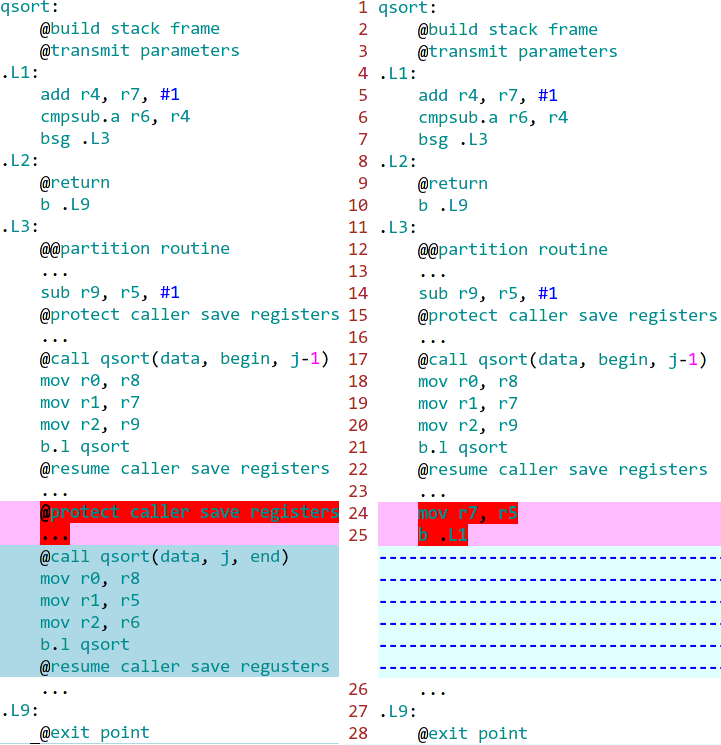
\includegraphics[scale=0.44]{tail_recursion.png}
	\captionof{figure}{尾递归示例}
	\label{fig:tailrecursion}
\end{center}
可以看出,在第二个\verb|qsort|的调用时(24行-30行),进行尾递归优化的程序(右)直接将新值\verb|j|传入被修改的参数\verb|begin|所在的寄存器\verb|r7|中,然后无条件跳转到了函数的正文标号\verb|.L1|。节省了保存、恢复现场以及新调用建立栈帧的指令。\\
{\it \anchor 有关尾递归优化的代码,请参阅:\verb|gen_target_code.c|}\\

\subsection{指令调度}
\label{assembledispatch}
根据Unicore32指令系统体系结构,除了载入和运算指令可能产生的数据相关无法转发,需要等待一个cycle以外,其它指令的数据相关均已通过转发解决。指令调度的目的是减少甚至消除因载入指令而造成的数据相关。

\paragraph*{算法}
\begin{enumerate}
	\item 在目标代码上划分基本块(以跳转指令和标签作为标记)。指令调度在基本块内完成。
	\item 对每个基本块,根据指令间的数据依赖关系,建立数据依赖图。若指令$i$的源操作数依赖于指令$j$的执行结果,则建立$j$到
$i$的一条边。
	\item 根据数据依赖图,进行变种的拓扑排序:扫描块中所有指令。遇到\verb|ldw|指令,则开始执行所有\verb|ldw|指令依赖的指令(即在图上可达这条\verb|ldw|指令的指令);之后,从所有本块中未执行过的指令中取出一条入度为0的指令(不依赖于任何指令),排在这条\verb|ldw|指令后面。特别地,这条指令的源操作数应该尽量和\verb|ldw|指令的目标操作数不相等。
	\item 扫描一遍\verb|ldw|指令之后,所有可能调开的\verb|ldw|指令都已经被调开。再对未执行的指令进行拓扑排序即可。
\end{enumerate}
\paragraph*{示例}
下面是一段汇编指令:
\begin{verbatim}
	ldw	r4, [r6+], #4
	add	r5, r4, r5
	ldw	r4, [r6+], #4
	sub	r4, r4, r5
	ldw	r30, [r27+], #-4
\end{verbatim}
它的依赖关系图如下:
\begin{center}
	\includegraphics[scale=0.35]{assemble_rely_graph.png}
\end{center}
调度后的指令序列:
\begin{verbatim}
	ldw	r4, [r6+], #4
	add	r5, r4, r5
	ldw	r4, [r6+], #4
	ldw	r30, [r27+], #-4
	sub	r4, r4, r5
\end{verbatim}
{\it \anchor 有关指令调度的代码,请参阅:\verb|instruction_dispatch.c|}\\
\section{谬误与陷阱}
\label{tarpitc3}
\subsection*{编译优化与结果正确性}
教科书上对编译优化的要求是:以\emph{正确}为前提,尽可能地提升目标代码的效率。然而在实践中,存在着一些对“正确”定义不清的灰色地带,如果一味地追求绝对正确,将大大损失性能。例如对如下的一段C代码:
\begin{lstlisting}
void f(int* p)
{
	*p = 1;
}
int main()
{
	int a,b,c,*p;
	p = &b;
	p += 1;
	//*p = c 
	f(p);
}
\end{lstlisting}
按照原则上来说,如果一个程序员对他所面对的目标机器足够了解的话,\verb|p += 1|的使用也许是为了指向\verb|a|(或\verb|c|),因此在调用函数\verb|f|的时候应当将\verb|a|(或\verb|c|)的值同步到内存中以保证“正确”。

然而\verb|unicore32-linux-gcc|使用\verb|-O2|编译参数的结果却是错误的:它没有做任何的访存操作来保护内存和寄存器的同步。

原因是\verb|gcc|在性能和“绝对正确”之间做出了权衡:应该由程序员而不是编译器应该保证这种极为特殊的情况的正确性。

这样做所换来的性能提升也是可观的:在不考虑指针计算的情况下,简单的数据流指针分析就能够精确地得到应该同步的变量。

为了在绝大部分情况下提高性能,MiniC也要求这种特殊情况由程序员自行保证。(去掉上面代码中的注释即可)

当然,在“保证绝对正确”的编译选项下,情况又不同了,这时候就算牺牲性能也要保证没有任何差错。


